%!TEX root = report.tex
\section{Experimental Results}

\subsection{Reference frames}
Two reference frames are used in the experiments. First, there is the point reference frame, in which the visual localization is done. 
In this frame, the x axis is defined to point from the first to the second reference point (\textit{ref basis} in Figure \ref{fig:res1_room} and \ref{fig:res2_room} ) and the z axis points out of the floor.
For visualization purposes, a margin in x and y direction is added to these points, so the origin is slightly offset from the basis line (see \textit{ref origin} in Figures \ref{fig:res1_room} and \ref{fig:res2_room}).

\subsection{Experiment in BC building hall (Atrium)}
The first experiments were done in the Atrium of the BC building, with 5 orange reference points for extrinsic calibration and a bottle as a target point instead of the robot.
This setup is characterized by a small height difference between the reference points (height 20 mm) and the target point (height 160 mm). 
The cameras are placed at a height of around 2 meters which leads to bottom-down views for all cameras (Figure \ref{fig:res0_img139} and \ref{fig:res0_img141}).
The resulting error of the bottle position is less than 18mm for all camera combinations and goes down to 5.8mm in 3D (cameras 139, 141, 145) or 4 mm in 2D with fixed height (cameras 139, 143) (see Figure~\ref{fig:res0_err}). 

\begin{figure}
    \centering
    \begin{subfigure}{0.49\linewidth}
        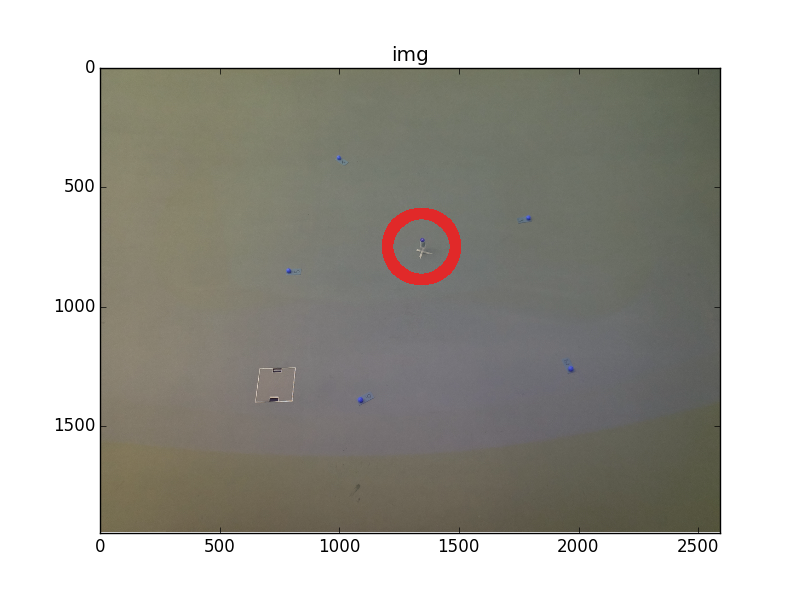
\includegraphics[width=\linewidth]{files/res0_img139.png}
        \caption{View from camera 139.}
        \label{fig:res0_img139}
    \end{subfigure}
    \begin{subfigure}{0.49\linewidth}
        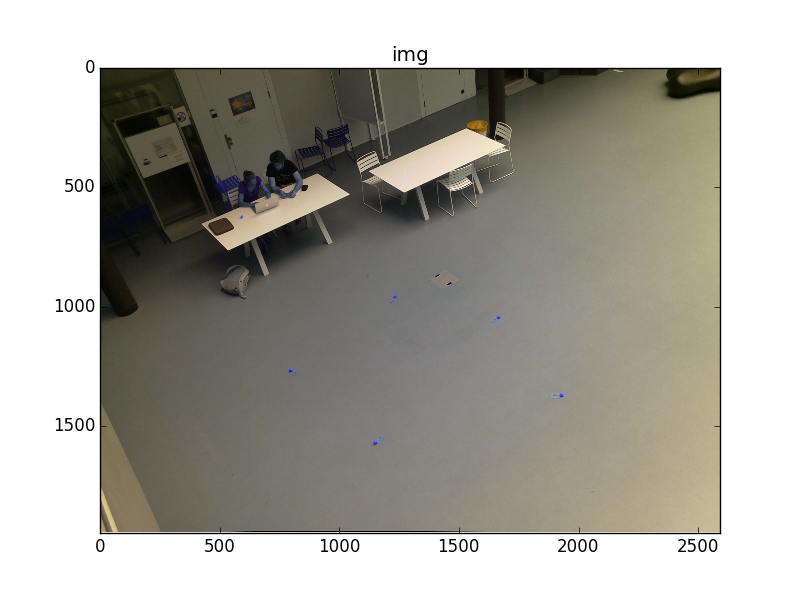
\includegraphics[width=\linewidth]{files/res0_img141.png}
        \caption{View from camera 141. }
        \label{fig:res0_img141}
    \end{subfigure}
    \caption{Experiment in Atrium: camera views with 5 blue reference points and the bottle as target point in view 139.}
    \label{fig:res0_views}
\end{figure}


\subsection{Experiment in BC329 with reference points}

A second experiment was performed in a more realistic setting in BC room 329, using 6 reference points for extrinsic calibration and the real robot as target point (see Figure \ref{fig:res1_img}). 
In addition to the visual localization, odometry was used to evaluate the position of the robot.
\begin{figure}
    \centering
    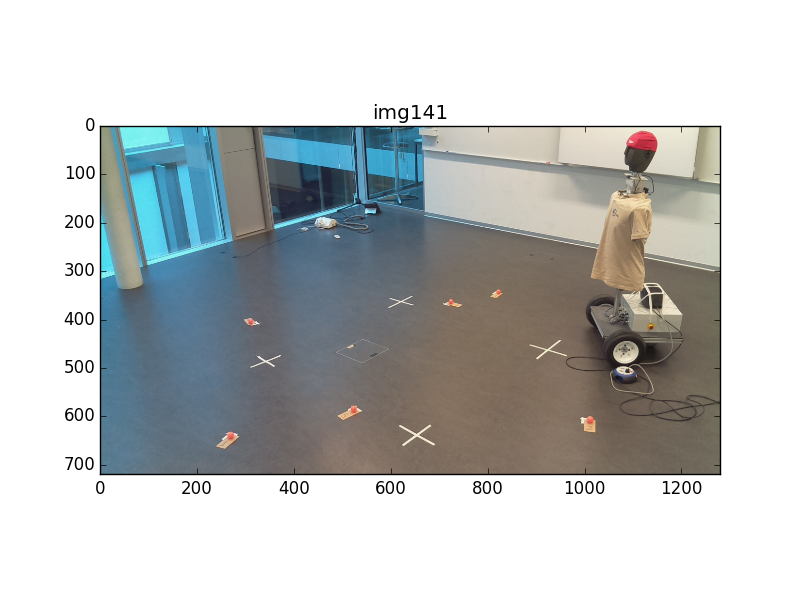
\includegraphics[width=.6\linewidth]{files/res1_img141.png}
    \caption{Experiment with reference points: view from camera 141.}
    \label{fig:res1_img}
\end{figure}
The performance of odometry was measured at 3 positions but because of technical issues, visual localization could only be performed at one position. 
The robot's real positions, measured positions within the room, and the placement of the cameras are illustrated in Figure \ref{fig:res1_room}.
The position calculated by visual localization is quite far from the real positions, which can be more clearly seen in Figure \ref{fig:res1_combi}. 

\begin{figure}
    \centering
    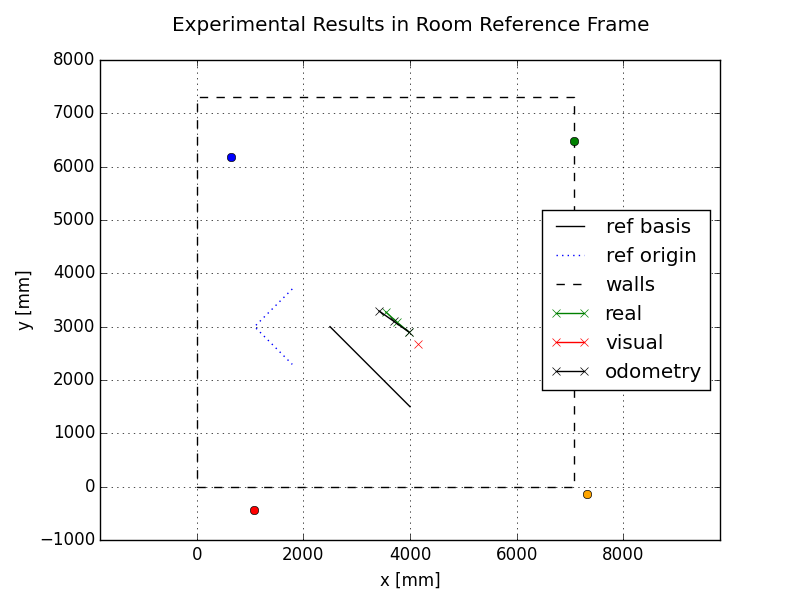
\includegraphics[width=.8\linewidth]{files/res1_room.png}
    \caption{Experiment with reference points: summary of results in room reference frame (Camera numbering: blue 139, red 141, green 143, orange 145).}
    \label{fig:res1_room}
\end{figure}

The best result is obtained with the camera combination (141,143); all other combinations give significantly higher error.
The resulting error (46 mm) from the best camera combination is still significantly higher than for the experiments in the Atrium, as the view is much less bottom-down, so small errors in height lead to large lateral errors.
A more closer look of the results reveils that the height of the robot is very badly determined when camera 145 is used. This is not a result of errors in the calculation of the position of the camera, which is as accurate as the others (Figure \ref{fig:res1_room}, orange point). 
It could be that its position relative to the robot is poorly chosen, as it is comparatively close to the robot head meaning that the calculated position is very sensitive to small changes in the robot position within the image (see Figure \ref{fig:res1_img145}).

\begin{figure}
    \centering
    \begin{subfigure}{0.49\linewidth}
        \centering
        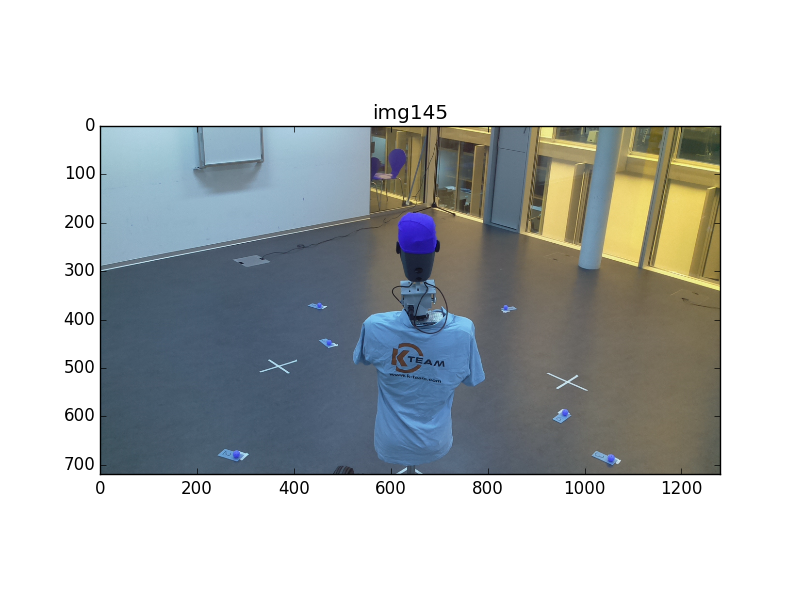
\includegraphics[width=\linewidth]{files/res1_img145.png}
        \caption{View from camera 145.}
        \label{fig:res1_img145}
    \end{subfigure}
    \begin{subfigure}{0.49\linewidth}
        \centering
        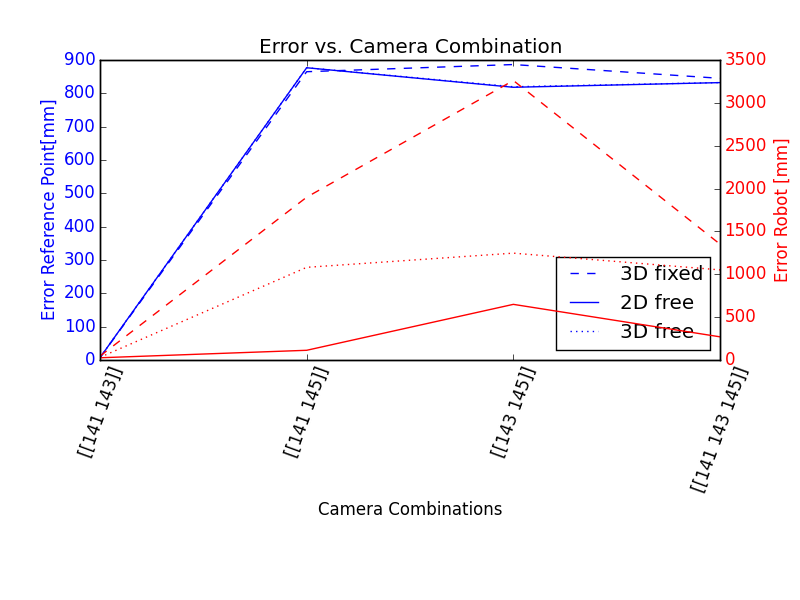
\includegraphics[width=\linewidth]{files/res1_combi_4.png}
        \caption{2D and 3D errors of 4th reference point and robot at the first position.}
        \label{fig:res1_combi}
    \end{subfigure}
    \caption{Experiment with reference points: view of badly positioning camera 145 and results of visual localization.}
    \label{fig:experiment1}
\end{figure}



\subsection{Experiment 1 in BC329 with checkerboard}

A third experiment was performed in the same setting as above but using the checkerboard algorithm for extrinsic calibration instead of reference points (see Figures \ref{fig:res2_image_143} and  \ref{fig:res2_output_143}). 
The visual localization was performed at two locations and its results were significantly better than for the previous experiment. 

\begin{figure}
    \centering
    \begin{subfigure}{0.49\linewidth}
        \centering
        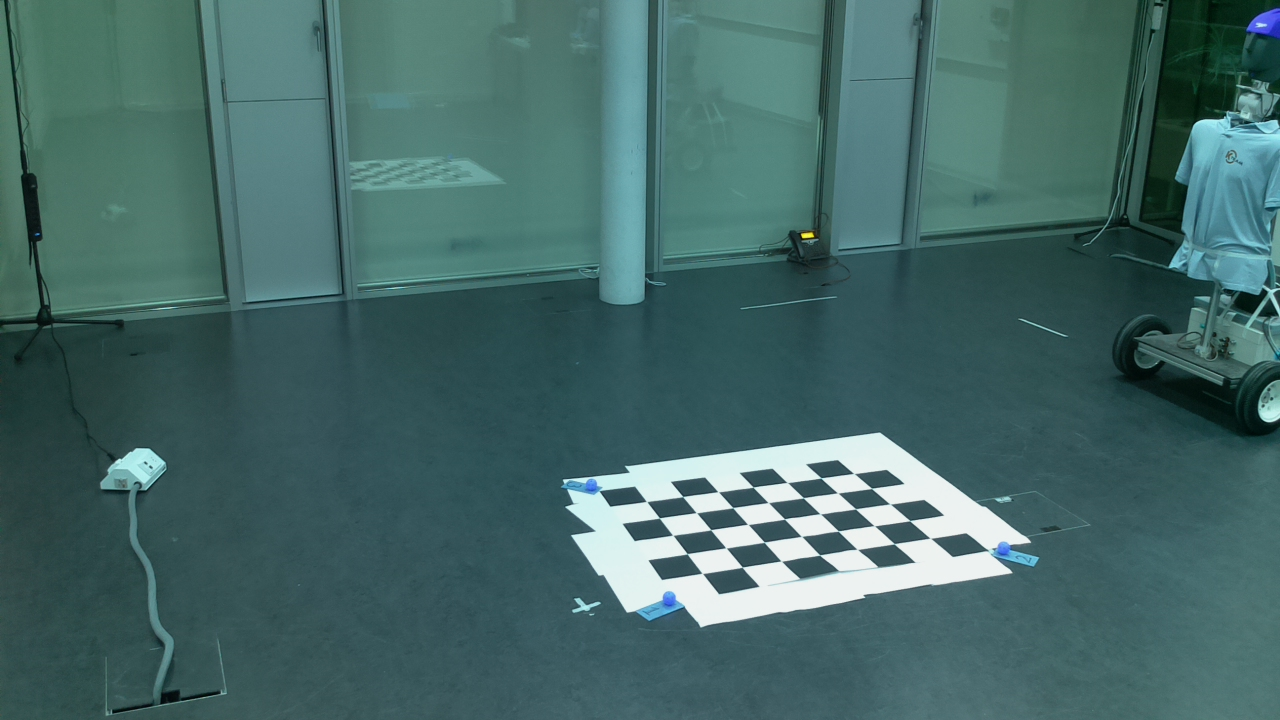
\includegraphics[width=\linewidth]{files/res2_image_143.png}
        \caption{input: original view from camera 143.}
        \label{fig:res2_image_143}
    \end{subfigure}
    \begin{subfigure}{0.49\linewidth}
        \centering
        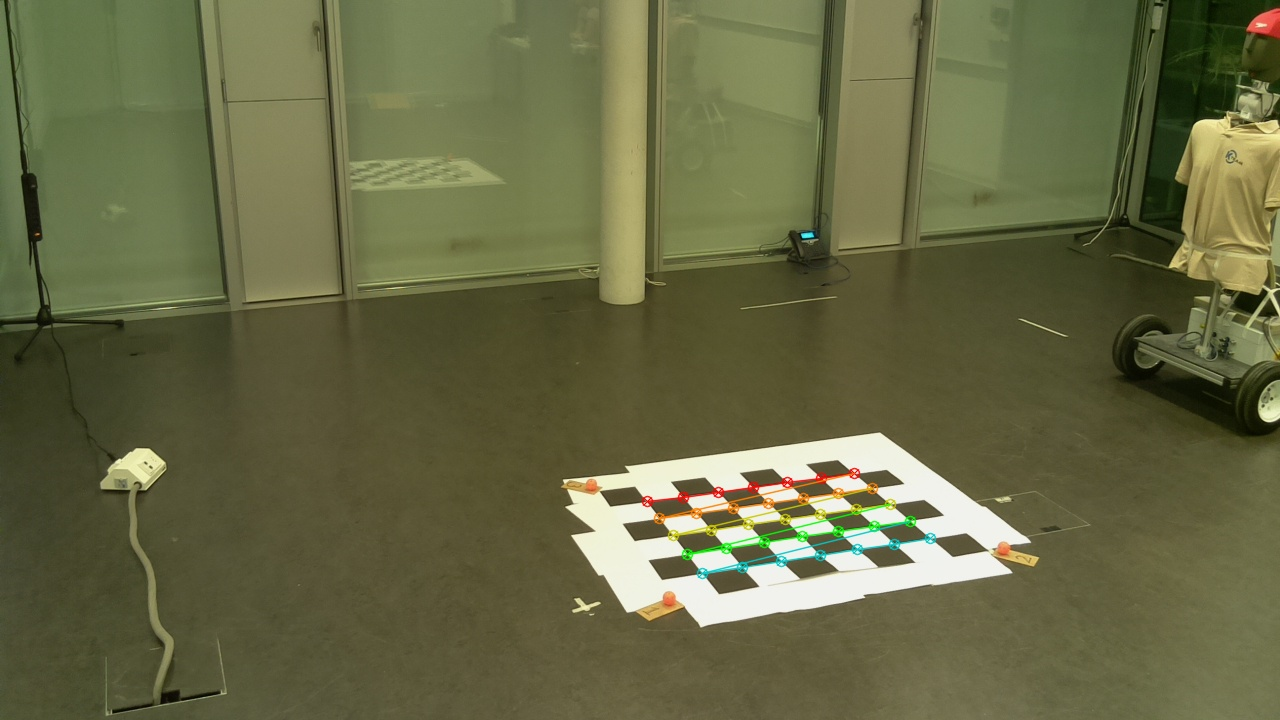
\includegraphics[width=\linewidth]{files/res2_output_143.jpg}
        \caption{output: view with detected checkerboard corners.}
        \label{fig:res2_output_143}
    \end{subfigure}
    \caption{Experiment 1 with checkerboard: input and output of extrinsic calibration.}
    \label{fig:experiment2}
\end{figure}

The robot position errors are shown in Figure \ref{fig:res2_combi}. Two tendencies can be observed:
including the camera 145 tends to spoil the result, while an increasing number of cameras tends to improve the result. The best result is obtained for the combination (141, 143, 145) of an error of around 80mm.
For the second position, only cameras 139 and 141 could be considered because of technical issues and they led to an error of around 100mm for both fixed- and free-height algorithms. 
\begin{figure}
    \centering
    \begin{subfigure}{0.49\linewidth}
        \centering
        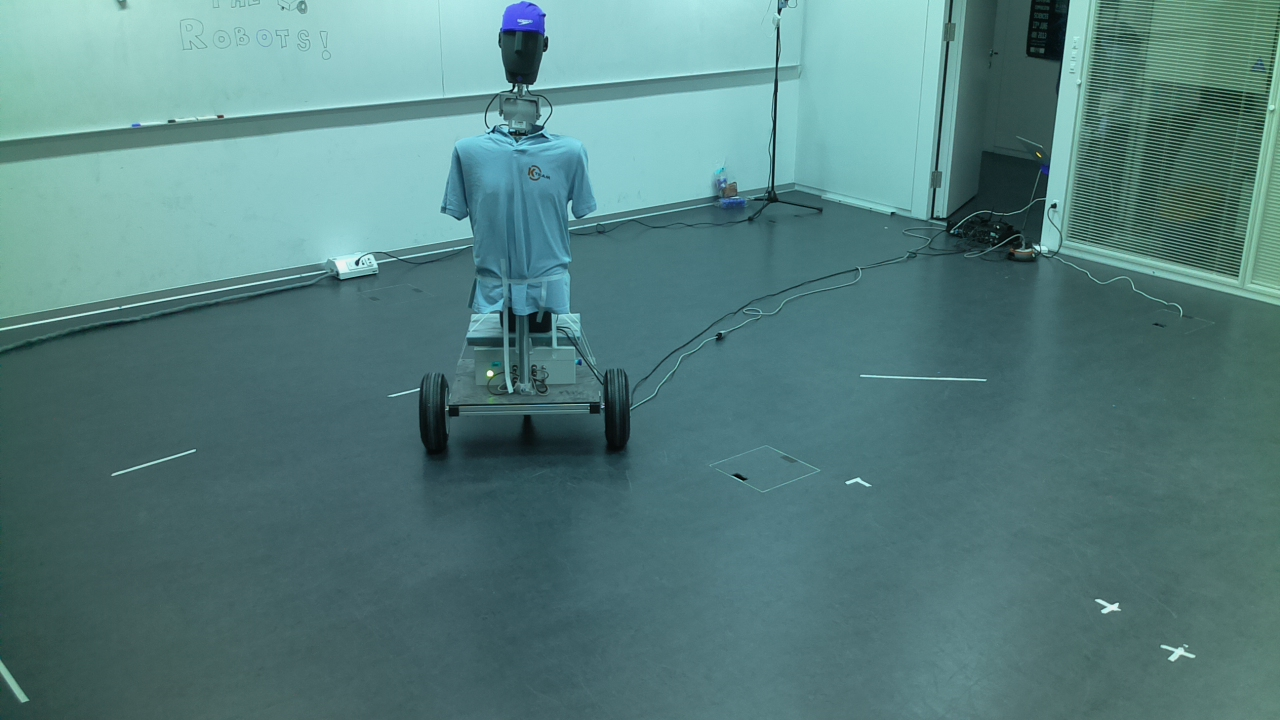
\includegraphics[width=\linewidth]{files/res2_0_image_141.png}
        \caption{View from camera 141 with robot.}
        \label{fig:res2_0_image_141}
    \end{subfigure}
    \begin{subfigure}{0.49\linewidth}
        \centering
        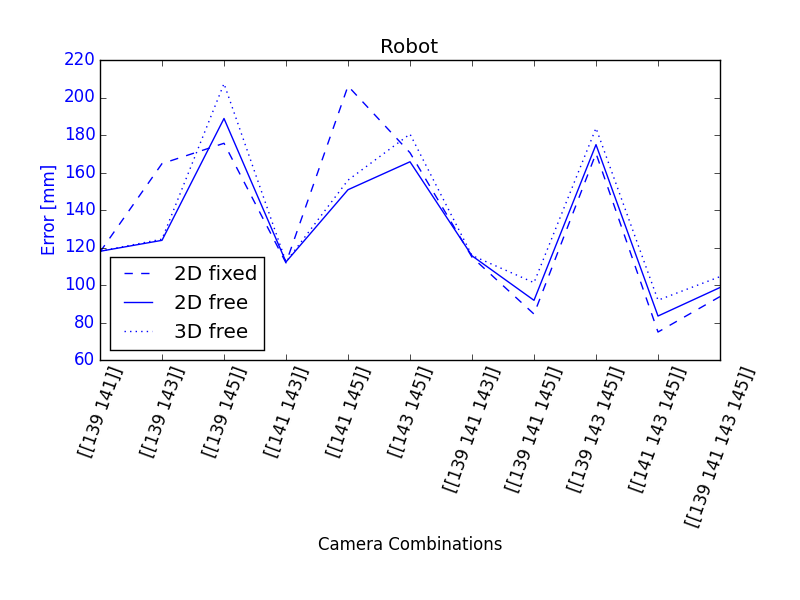
\includegraphics[width=\linewidth]{files/res2_combi_rob.png}
        \caption{2D and 3D errors of robot.}
        \label{fig:res2_combi}
    \end{subfigure}
    \caption{Experiment 1 with checkerboard: view of camera 141 and results of visual localization.}
    \label{fig:experiment2_2}
\end{figure}

In general, the height was very accurately determined to be 1615mm at the first position and 1640mm at the second position (Table \ref{tab:res2_errors}).
The results and the camera positions are shown in Figure \ref{fig:res2_room}.

\begin{table}
\begin{center}
\caption{Experiment 1 with checkerboard: positions obtained with free-height and fixed-height algorithm.}
\begin{tabular}{lcccccc}
\toprule
    & \multicolumn{3}{c}{\textbf{Position 1}} & \multicolumn{3}{c}{\textbf{Position 2}} \\
\midrule
& \textbf{Real} & Free & Fixed & \textbf{Real} & Free & Fixed \\
x   & \textbf{4299} & 4354 & 4331 & \textbf{4014} & 4113 & 4112  \\
y   & \textbf{4304} & 4222 & 4237 & \textbf{4596} & 4579 & 4580 \\
z   & \textbf{1650} & 1615 & 1650 & \textbf{1650} & 1640 & 1650 \\
\bottomrule
\end{tabular}
\label{tab:res2_errors}
\end{center}
\end{table}

\begin{figure}
    \centering
    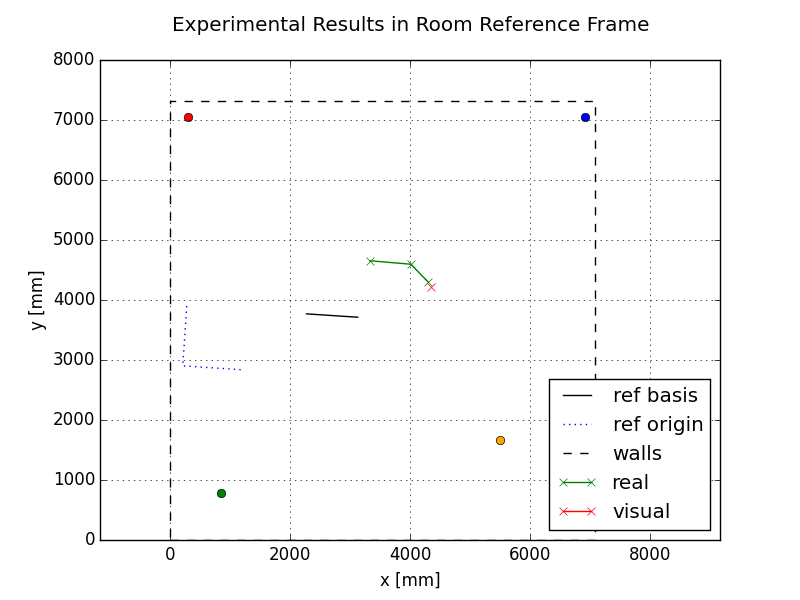
\includegraphics[width=.6\linewidth]{files/res2_room.png}
    \caption{Experiment 1 with checkerboard: summary of results in room reference frame (Camera numbering: blue 139, red 141, green 143, orange 145).}
    \label{fig:res2_room}
\end{figure}


\subsection{Experiment 2 in BC329 with checkerboard}

\subsubsection{Visual and odometry results}

\begin{figure}
    \centering
    \begin{subfigure}{0.7\linewidth}
        \centering
        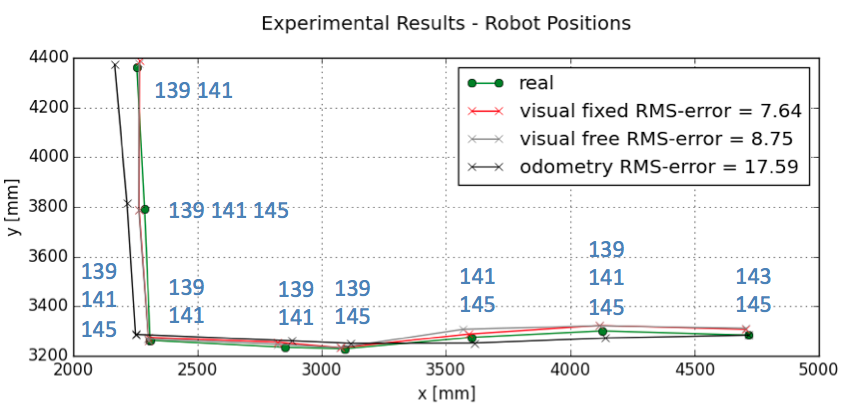
\includegraphics[width=\textwidth]{files/res3_best_err.png}
        \caption{Robot positions using best camera combination.}
        \label{fig:res3_best_err}
    \end{subfigure} 
    \begin{subfigure}{0.8\linewidth}
        \centering
        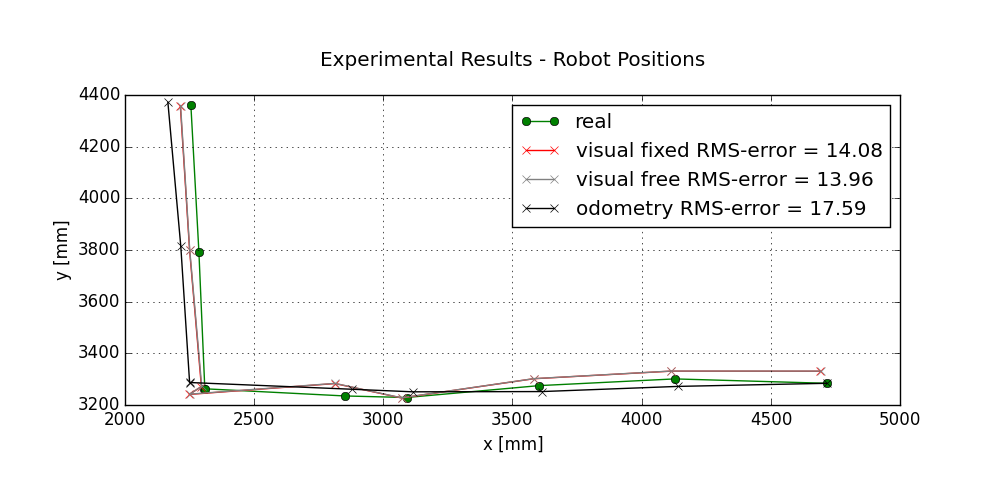
\includegraphics[width=\textwidth]{files/res3_all_err.png}
        \caption{Robot positions using all cameras.}
        \label{fig:res3_all}
    \end{subfigure} 
    \caption{Experiment 2 with checkerboard: Robot positions.}
    \label{fig:res3_err}
\end{figure}

\begin{figure}
    \centering
    \begin{subfigure}{0.49\linewidth}
        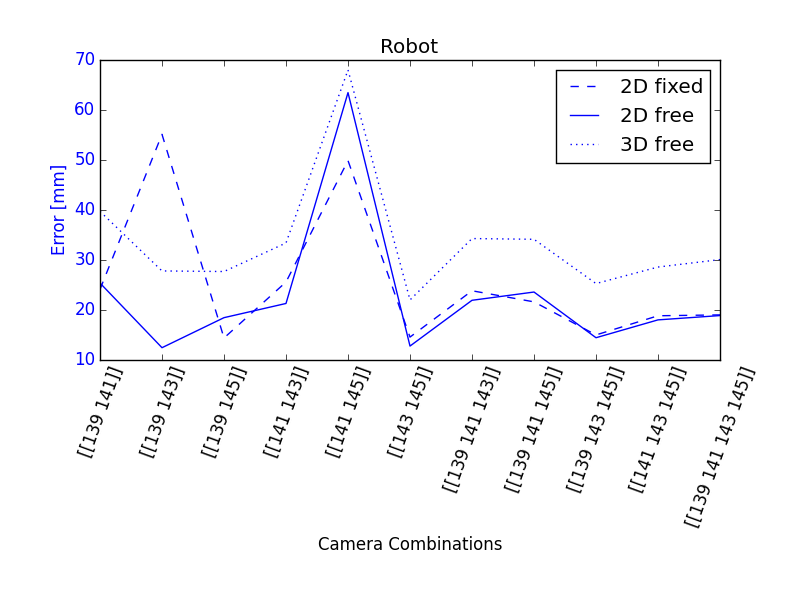
\includegraphics[width=\textwidth]{files/res3_err3}
        \caption{Position 3}
        \label{fig:res3_err3}
    \end{subfigure}
    \begin{subfigure}{0.49\linewidth}
        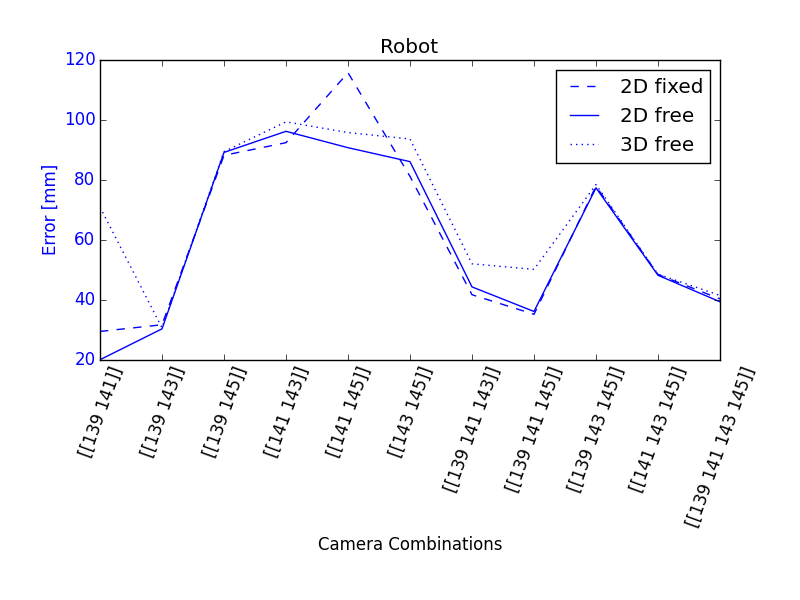
\includegraphics[width=\textwidth]{files/res3_err8}
        \caption{Position 8}
        \label{fig:res3_err8}
    \end{subfigure}
    \caption{Experiment 2 with checkerboard: 2D and 3D errors of robot at two example positions.}
    \label{fig:res3_errors}
\end{figure}


Figure \ref{fig:res3_best_err} shows the robot's real positions compared to the results of the visual localization and the odometry calculations. 
The camera combination resulting in each visual positioning is noted next to the respective points. 
As expected, the odometry continuously shifts away from the real positions, leading to a mean error of 17.59 mm. 
The visual positioning is comparatively more accurate with a mean error of less than a centimeter. 
If the real height of the robot is specified, the obtained error goes down to 7.64 mm.
This precision is slightly overestimated as, in real experiments, the robot's real position and the resulting best camera combination will not be known. 
As Figures \ref{fig:res3_err3} and \ref{fig:res3_err8} suggest, using all four cameras might not always lead to the best solution (in fact, it never does, as shown in Figure \ref{fig:res3_best_err}), but it always leads to a reasonable solution compared to other combinations whose results are much more varied (e.g. combination (139,145)). 
Therefore, it could be considered to always use all four cameras for positioning. 
The results using this approach are shown in Figure \ref{fig:res3_all}.

Table \ref{tab:res3_errors} visualizes how the size of the robot head limits the precision of the visual localization results. 
The two positions considered are position 5 and 6 which differ mainly in the orientation of the robot (its real position only changes by around 5 mm).
The results of the visual localization with both fixed and free height differ by 50 mm however. 
This result indicates that due to the geometry of the robot head, one cannot precisely derive the real position from its image coordinates.

\begin{table}
\begin{center}
\caption{Experiment 2 with checkerboard: positions 5 and 6 with free-height and fixed-height algorithm.}
\begin{tabular}{lcccccc}
\toprule
& \multicolumn{2}{c}{Free} & \multicolumn{2}{c}{Fixed} & \multicolumn{2}{c}{Real} \\
Pos & 5 & 6 & 5 & 6 & 5 & 6\\
\midrule
x&2276& 2302& 2275& 2302 & 2284 & 2289\\
y&3218& 3260& 3218& 3261 & 3243 & 3242\\
z&1644& 1634& 1650& 1650 & 1650 & 1650\\
\midrule
error & \multicolumn{2}{c}{\textbf{50.4}}&\multicolumn{2}{c}{\textbf{50.8}} &\multicolumn{2}{c}{\textbf{5}}\\
\bottomrule
\end{tabular}
\label{tab:res3_errors}
\end{center}
\end{table}

A summary of the all obtained positions including the camera's theoretical and calculated positioning is shown in Figure \ref{fig:res3_room}.

\begin{figure}
    \centering
    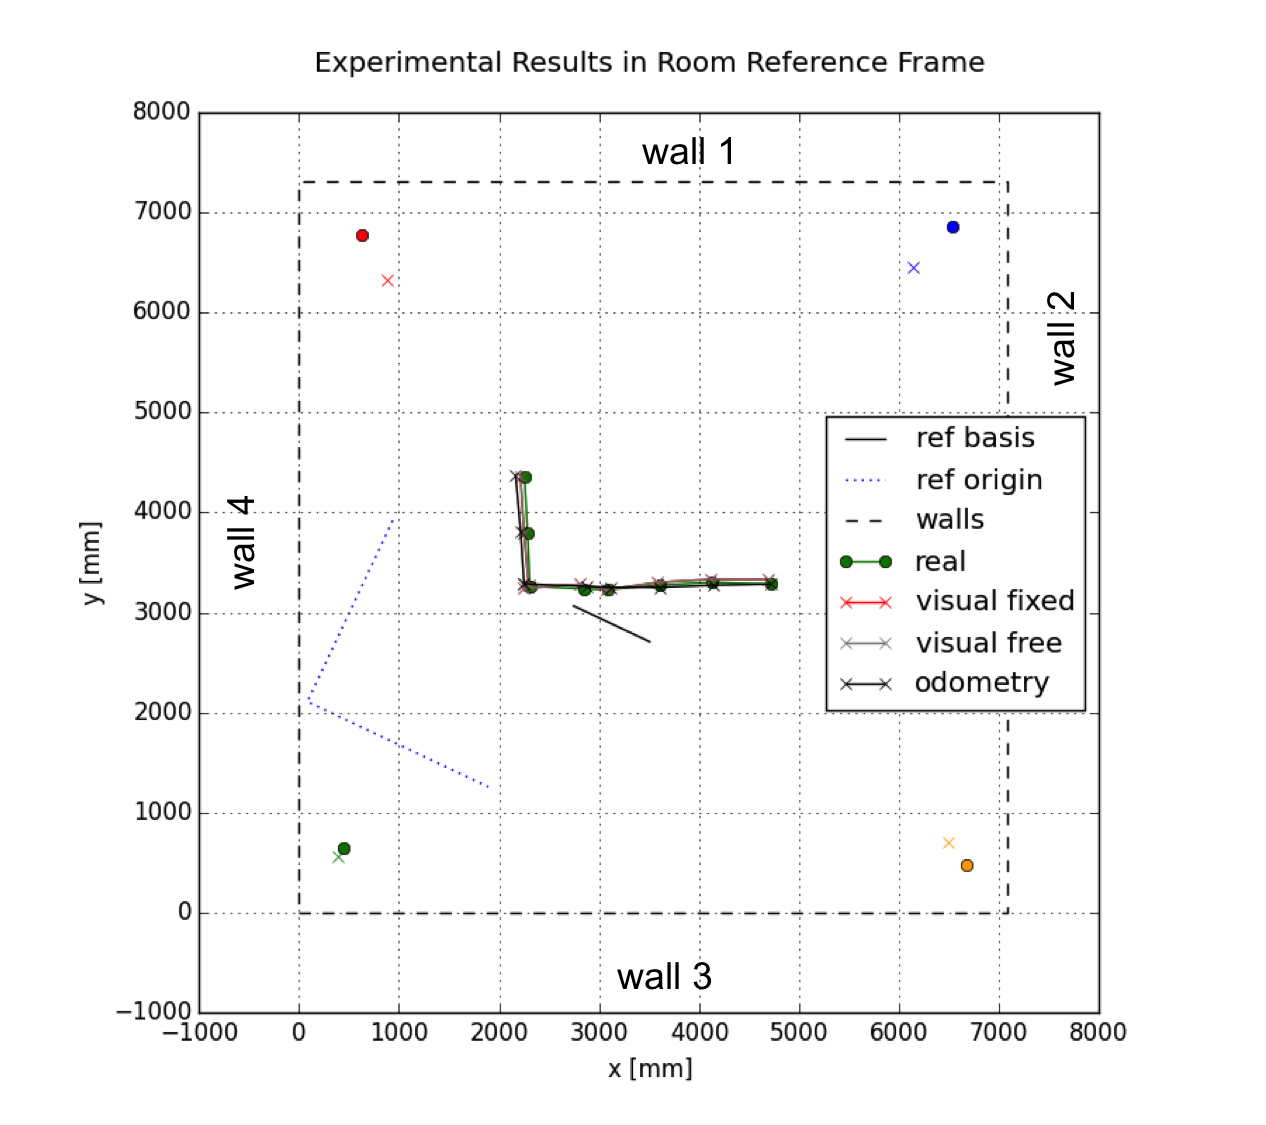
\includegraphics[width=.8\linewidth]{files/res3_all_room2.png}
    \caption{Experiment 2 with checkerboard: summary of results in room reference frame (Camera numbering: blue 139, red 141, green 143, orange 145). 'o' and 'x' denote the real and calculated positions respectively.}
    \label{fig:res3_room}
\end{figure}
%!TEX root=report.tex
\subsubsection{Impulse responses}

The room impulse responses were computed for all positions following the procedure described in § \ref{sec:analysis}. The same assumptions on the speaker and microphones were made, however this time the echo created by the ceiling was considered as well.

The signal is quite noisy and the peaks are not easily discernible, but the primary echo, coming directly from the speaker, and the echo created by the ceiling are clearly visible in all responses. 
There is a small delay between the expected ceiling echo and the detected one which could be due to a imprecision in the latency measurement or because the speed of sound was not calibrated with the temperature.

Since the first steps of the robot were parallel to walls 1 and 3 and the last steps to walls 2 and 4 (see Figure \ref{fig:res3_room} for wall numbering), it would be expected that the peaks corresponding to those walls should remain constant while the other peaks should be moving according to the robot's movement. 
This phenomenon is not clearly discernible between positions 1 and 2 as shown in Figures \ref{fig:rir_1} and \ref{fig:rir_2}. It is more clear between positions 7 and 8, where the peak corresponding to wall 1 moves earlier in the signal as expected.

%An attempt was made to identify this movement using the cross-correlation between the two impulse responses at positions 7 and 8 (Figure \ref{fig:corr78}). Assuming that both responses are identical besides the two moving peaks, one would expect 2 peaks in the cross-correlation, corresponding to the time delay of the echoes induced by the robot's movement.
\begin{figure}
    \centering
    \begin{subfigure}{0.49\linewidth}
        \centering
        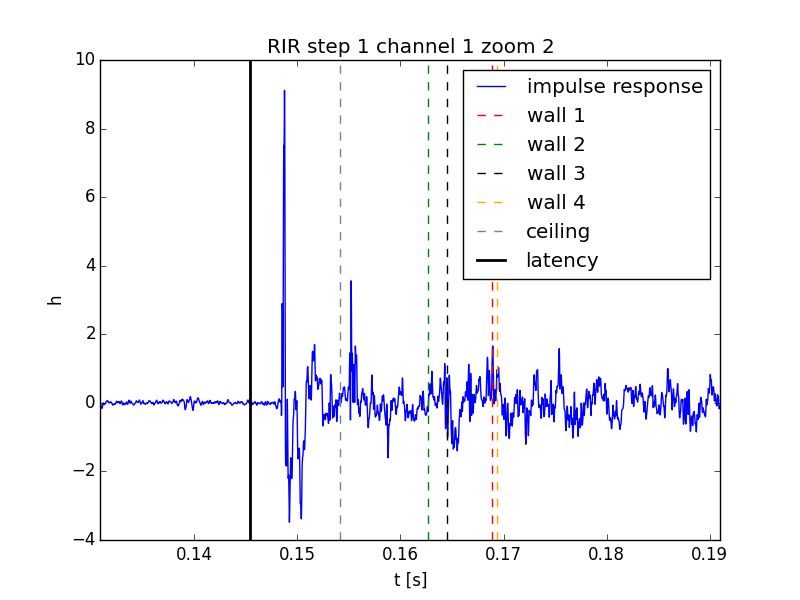
\includegraphics[width=\linewidth]{files/1_1_filt_zoom2.png}
        \caption{Position 1.}
        \label{fig:rir_1}
    \end{subfigure}
    \begin{subfigure}{0.49\linewidth}
        \centering
        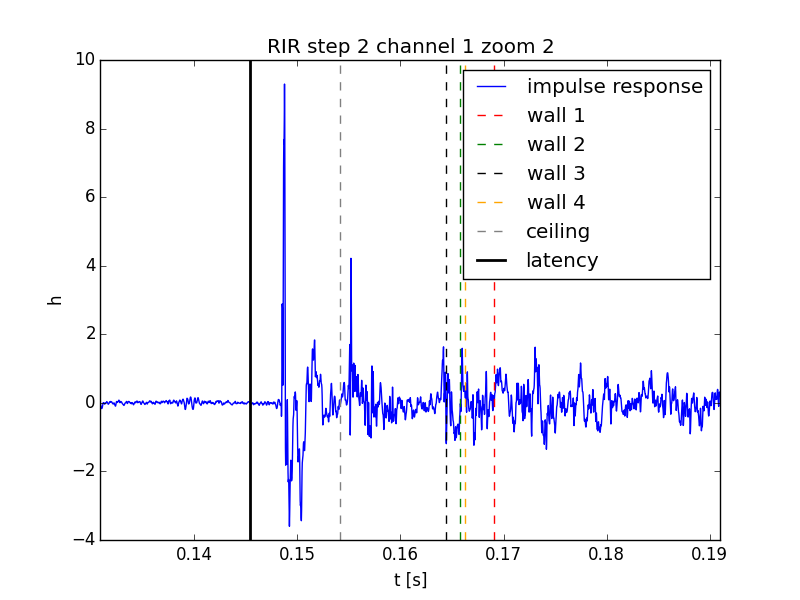
\includegraphics[width=\linewidth]{files/2_1_filt_zoom2.png}
        \caption{Position 2.}
        \label{fig:rir_2}
    \end{subfigure}
    \begin{subfigure}{0.49\linewidth}
        \centering
        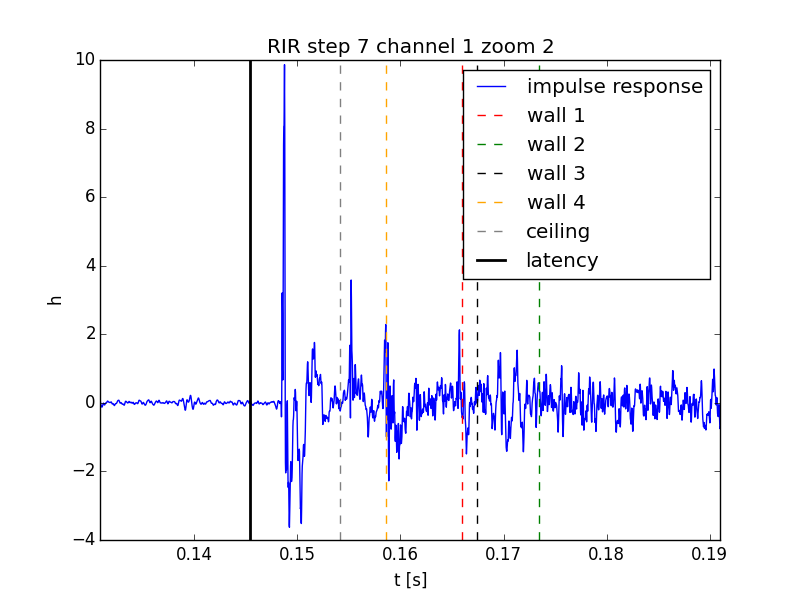
\includegraphics[width=\linewidth]{files/7_1_filt_zoom2.png}
        \caption{Position 7.}
        \label{fig:rir_7}
    \end{subfigure}
    \begin{subfigure}{0.49\linewidth}
        \centering
        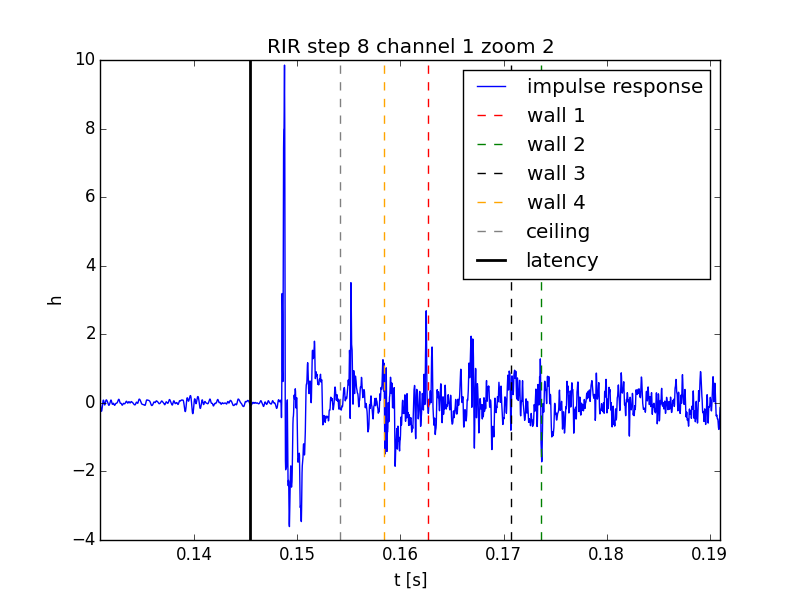
\includegraphics[width=\linewidth]{files/8_1_filt_zoom2.png}
        \caption{Position 8.}
        \label{fig:rir_8}
    \end{subfigure}
    \caption{Room impulse responses at Positions 1,2,7 and 8.}
    \label{fig:rir}
\end{figure}

%\begin{figure}
    %\centering
    %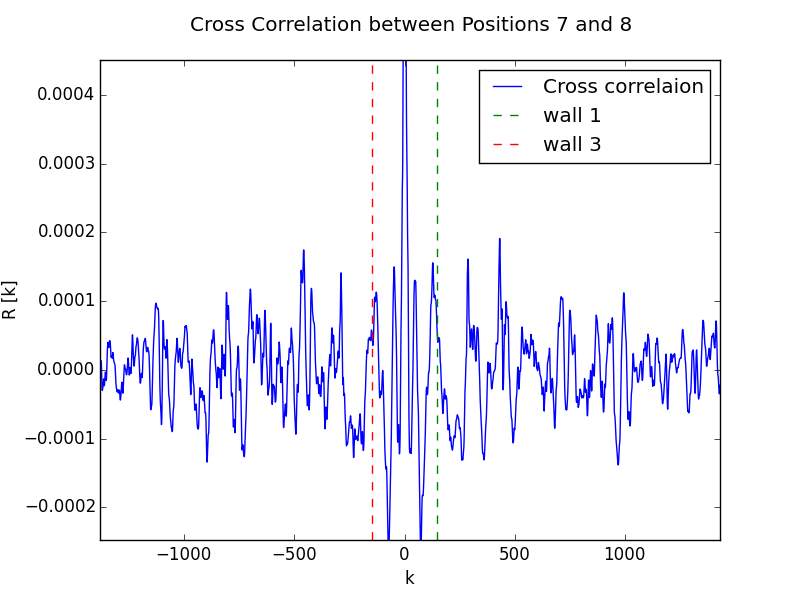
\includegraphics[width=0.6\linewidth]{files/CrossCorr78}
    %\caption{Cross-correlation between positions 7 and 8.} 
    %\label{fig:corr78}}
%\end{figure}


